\section{Техническое задание}
\subsection{Основание для разработки}

Основанием для разработки является задание на преддипломную (производственную) практику "Корпоративный портал учёта рабочего времени. Клиентская часть".

\subsection{Цель и назначение разработки}

Основной задачей является разработка и внедрение корпоративного портала для учёта рабочего времени для организации ООО "НОРБИТ".

Посредством внедрения планируется вести учёт рабочего времени сотрудников, отслеживать задачи и проекты пользователей.

Задачами данной разработки являются:
\begin{itemize}
\item создание информационных разделов сайта;
\item реализация формы для авторизации;
\item реализация страницы редактирования информации о проектах;
\item реализация страницы редактирования информации о задачах;
\item реализация страницы редактирования информации о проводках;
\item реализация страницы просмотра информации о проводках;
\item создание системы поиска/фильтрации содержимого страницы просмотра.
\end{itemize}

\subsection{Требования пользователя к web-сайту}

\subsubsection{Требования к интерфейсу}
Сайт должен включать в себя:
\begin{itemize}
    \item навигацию по разделам;
    \item страницу авторизации;
    \item страницу редактора с разделами редактирования проектов, задач и т.д.;
	\item страницу просмотра.
\end{itemize}

Макет интерфейса сайта представлен на рисунке ~\ref{fig:templ}.

\begin{figure}[H]
	\centering
	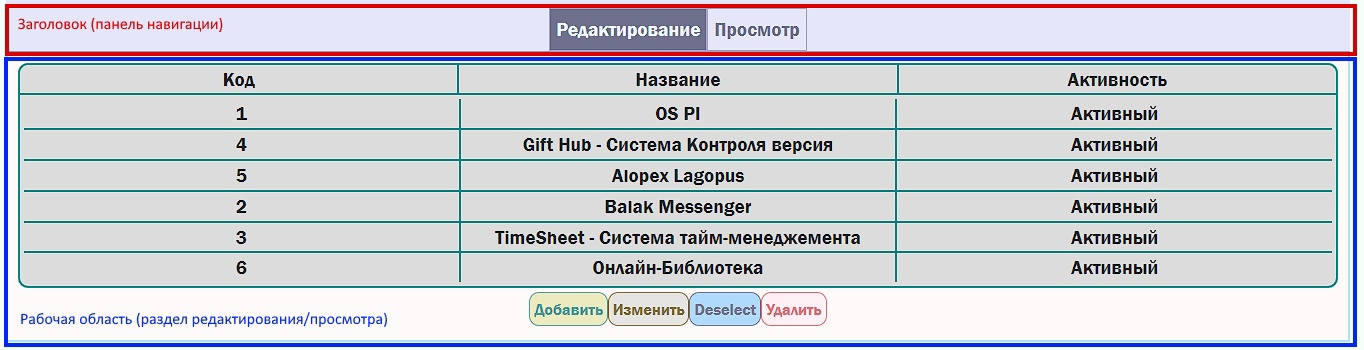
\includegraphics[width=1\linewidth]{images/templ}
	\caption{Макет интерфейса сайта}
	\label{fig:templ}
\end{figure}
%\vspace{-\figureaboveskip} % двойной отступ не нужен (можно использовать, если раздел заканчивается картинкой)

\subsubsection{Функциональные требования}
Пользователю должны быть доступны следующие функции web-сайта:
\begin{enumerate}
	\item Добавление информации о проекте (задаче, проводках).
	\item Изменение информации о проекте (задаче, проводках).
	\item Удаление информации о проекте (задаче, проводках).
	\item Просмотр информации о проекте (задаче, проводках).
	\item Фильтрация выведенной информации по дате и времени.
\end{enumerate}


На рисунке~\ref{fig:precedents} в виде диаграммы прецедентов представлены функциональные требования к системе.


\begin{figure}[H]
	\centering
	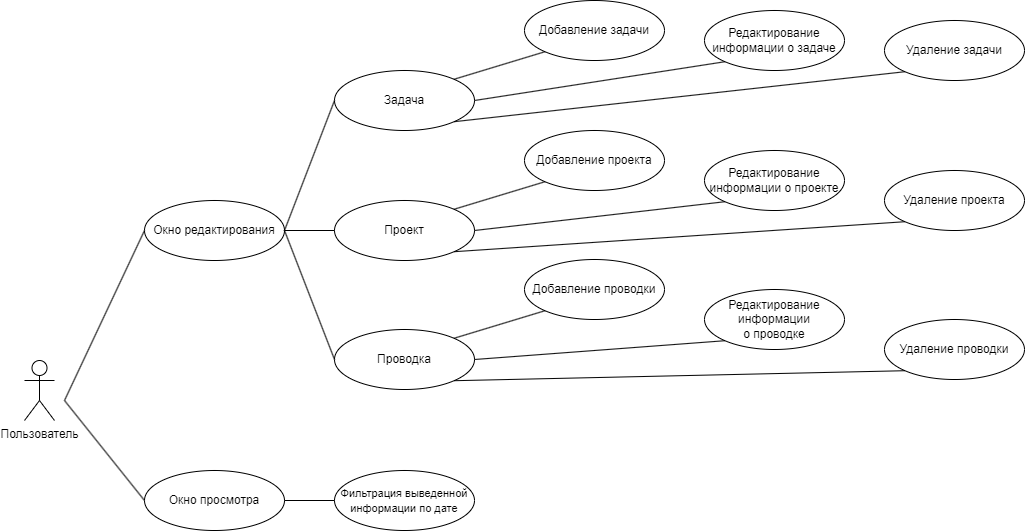
\includegraphics[width=1\linewidth]{images/precedents}
	\caption{Диаграмма прецедентов}
	\label{fig:precedents}
\end{figure}
%\vspace{-\figureaboveskip} % двойной отступ не нужен (можно использовать, если раздел заканчивается картинкой)

\subsubsection{Варианты использования}
\paragraph{Вариант использования "<Авторизация">}
Заинтересованные лица и их требования: Пользователи веб-портала, которые хотят получить доступ к порталу учета рабочего времени.
Предусловие: Пользователь портала имеет данные для входа от своей учетной записи. Открыто окно авторизации.
Постусловие: Пользователь входит в систему.

Основной успешный сценарий:
\begin{enumerate}
	\item Пользователь вводит логин в поле для ввода логина
	\item Пользователь вводит пароль в поле для ввода пароля
	\item Пользователь нажимает кнопку "<войти>"
	\item Происходит отправка запроса на логирование к серверу 
	\item Сервер отправляет на frontend json файл с пользовательскими данными
	\item Загружается главная страница сайта.
\end{enumerate}

\paragraph{Вариант использования "<Добавление проекта">}
Заинтересованные лица и их требования: Пользователи веб-портала, которые хотят добавить новый проект.
Предусловие: Пользователь портала осуществил авторизацию и находится в системе. Открыто окно редактирования информации о проектах.
Постусловие: Таблица с проектами обновляется, добавляются новые записи.

Основной успешный сценарий:
\begin{enumerate}
	\item Пользователь нажимает кнопку "<добавить">
	\item Открывается диалоговое окно добавления проекта
	\item Пользователь вводит название проекта
	\item Пользователь вводит код проекта
	\item Диалоговое окно добавления проекта закрывается
	\item Происходит отправка запроса на добавление к серверу 
	\item Сервер возвращает сообщение об успешном добавлении информации
	\item Таблица с проектами обновляется, отображаются введённые ранее проекты и проект, добавленный пользователем.
\end{enumerate}

\paragraph{Вариант использования "<Редактирование проекта">}
Заинтересованные лица и их требования: Пользователи веб-портала, которые хотят изменить информацию о проекте.
Предусловие: Пользователь портала осуществил авторизацию и находится в системе. Открыто окно редактирования информации о проектах.
Постусловие: Таблица с проектами обновляется, изменяется информация о проекте, который редактировал пользователь.

Основной успешный сценарий:
\begin{enumerate}
	\item Пользователь выбирает проект, информацию о котором хочет изменить, одинарным щелчком мыши
	\item Пользователь нажимает кнопку "<изменить">
	\item Открывается диалоговое окно редактирования проекта
	\item Пользователь изменяет информацию о проекте по своему усмотрению
	\item Диалоговое окно редактирования проекта закрывается
	\item Происходит отправка запроса на изменение к серверу 
	\item Сервер возвращает сообщение об успешном обновлении информации
	\item Таблица с проектами обновляется, для проекта, изменённого пользователем, выводится новая информация.
\end{enumerate}

\paragraph{Вариант использования "<Удаление проекта">}
Заинтересованные лица и их требования: Пользователи веб-портала, которые хотят удалить информацию о проекте.
Предусловие: Пользователь портала осуществил авторизацию и находится в системе. Открыто окно редактирования информации о проектах.
Постусловие: Таблица с проектами обновляется, выбранный для удаления проект не отображается.

Основной успешный сценарий:
\begin{enumerate}
	\item Пользователь выбирает проект, информацию о котором хочет удалить, одинарным щелчком мыши
	\item Пользователь нажимает кнопку "<удалить">
	\item Выводится предупреждение с запросом подтверждения удаления
	\item Пользователь подтверждает удаление
	\item Происходит отправка запроса на удаление к серверу 
	\item Сервер возвращает сообщение об успешном удалении информации
	\item Таблица с проектами обновляется, выбранный пользователем для удаления проект не отображается.
\end{enumerate}

\paragraph{Вариант использования "<Отображение информации о задаче в окне редактирования">}
Заинтересованные лица и их требования: Пользователи веб-портала, которые хотят просмотреть или отредактировать информацию о задачах.
Предусловие: Пользователь портала осуществил авторизацию и находится в системе. Открыто окно редактирования информации о проектах.
Постусловие: Окно редактирования информации о проектах сворачивается, открывается окно редактирования информации о задачах.

Основной успешный сценарий:
\begin{enumerate}
	\item Пользователь двойным щелчком мыши по проекту открывает окно редактирования задач
	\item Происходит отправка запроса на вывод информации к серверу 
	\item Сервер возвращает информацию о задачах
	\item Полученная от сервера информация добавляется в таблицу в окне редактирования задач.
\end{enumerate}

\paragraph{Вариант использования "<Добавление задачи">}
Заинтересованные лица и их требования: Пользователи веб-портала, которые хотят добавить новую задачу.
Предусловие: Пользователь портала осуществил авторизацию и находится в системе. Открыто окно редактирования информации о задачах.
Постусловие: Таблица с задачами обновляется, добавляются новые записи.

Основной успешный сценарий:
\begin{enumerate}
	\item Пользователь нажимает кнопку "<добавить">
	\item Открывается диалоговое окно добавления задачи
	\item Пользователь вводит название задачи
	\item Диалоговое окно добавления задачи закрывается
	\item Происходит отправка запроса на добавление к серверу 
	\item Сервер возвращает сообщение об успешном добавлении информации
	\item Таблица с задачами обновляется, отображаются введённые ранее задачи и задача, добавленная пользователем.
\end{enumerate}

\paragraph{Вариант использования "<Редактирование задачи">}
Заинтересованные лица и их требования: Пользователи веб-портала, которые хотят изменить информацию о задаче.
Предусловие: Пользователь портала осуществил авторизацию и находится в системе. Открыто окно редактирования информации о задачах.
Постусловие: Таблица с задачами обновляется, изменяется информация о задаче, которую редактировал пользователь.

Основной успешный сценарий:
\begin{enumerate}
	\item Пользователь выбирает задачу, информацию о которой хочет изменить, одинарным щелчком мыши
	\item Пользователь нажимает кнопку "<изменить">
	\item Открывается диалоговое окно редактирования задачи
	\item Пользователь изменяет информацию о задаче по своему усмотрению
	\item Диалоговое окно редактирования задачи закрывается
	\item Происходит отправка запроса на изменение к серверу 
	\item Сервер возвращает сообщение об успешном обновлении информации
	\item Таблица с задачами обновляется, для задачи, изменённой пользователем, выводится новая информация.
\end{enumerate}

\paragraph{Вариант использования "<Удаление задачи">}
Заинтересованные лица и их требования: Пользователи веб-портала, которые хотят удалить информацию о задаче.
Предусловие: Пользователь портала осуществил авторизацию и находится в системе. Открыто окно редактирования информации о задачах.
Постусловие: Таблица с задачами обновляется, выбранная для удаления задача не отображается.

Основной успешный сценарий:
\begin{enumerate}
	\item Пользователь выбирает задачу, информацию о которой хочет удалить, одинарным щелчком мыши
	\item Пользователь нажимает кнопку "<удалить">
	\item Выводится предупреждение с запросом подтверждения удаления
	\item Пользователь подтверждает удаление
	\item Происходит отправка запроса на удаление к серверу 
	\item Сервер возвращает сообщение об успешном удалении информации
	\item Таблица с задачами обновляется, выбранная пользователем для удаления задача не отображается.
\end{enumerate}

\paragraph{Вариант использования "<Отображение информации о проводке">}
Заинтересованные лица и их требования: Пользователи веб-портала, которые хотят просмотреть или отредактировать информацию о проводках.
Предусловие: Пользователь портала осуществил авторизацию и находится в системе. Открыто окно редактирования информации о задачах.
Постусловие: Окно редактирования информации о задачах сворачивается, открывается окно редактирования информации о проводках.

Основной успешный сценарий:
\begin{enumerate}
	\item Пользователь двойным щелчком мыши по задаче открывает окно редактирования проводок
	\item Происходит отправка запроса на вывод информации к серверу 
	\item Сервер возвращает информацию о проводках
	\item Полученная от сервера информация добавляется в таблицу в окне редактирования проводок.
\end{enumerate}

\paragraph{Вариант использования "<Добавление проводки">}
Заинтересованные лица и их требования: Пользователи веб-портала, которые хотят добавить новую проводку.
Предусловие: Пользователь портала осуществил авторизацию и находится в системе. Открыто окно редактирования информации о проводках.
Постусловие: Таблица с проводками обновляется, добавляются новые записи.

Основной успешный сценарий:
\begin{enumerate}
	\item Пользователь нажимает кнопку "<добавить">
	\item Открывается диалоговое окно добавления проводки
	\item Пользователь вводит описание проводки
	\item Пользователь вводит количество часов, ушедшее на проводку
	\item Пользователь вводит дату проводки
	\item Диалоговое окно добавления проводки закрывается
	\item Происходит отправка запроса на добавление к серверу 
	\item Сервер возвращает сообщение об успешном добавлении информации
	\item Таблица с проводками обновляется, отображаются введённые ранее проводки и проводка, добавленная пользователем.
\end{enumerate}

\paragraph{Вариант использования "<Редактирование проводки">}
Заинтересованные лица и их требования: Пользователи веб-портала, которые хотят изменить информацию о проводке.
Предусловие: Пользователь портала осуществил авторизацию и находится в системе. Открыто окно редактирования информации о проводках.
Постусловие: Таблица с проводками обновляется, изменяется информация о проводке, которую редактировал пользователь.

Основной успешный сценарий:
\begin{enumerate}
	\item Пользователь выбирает проводку, информацию о которой хочет изменить, одинарным щелчком мыши
	\item Пользователь нажимает кнопку "<изменить">
	\item Открывается диалоговое окно редактирования проводки
	\item Пользователь изменяет информацию о проводке по своему усмотрению
	\item Диалоговое окно редактирования проводки закрывается
	\item Происходит отправка запроса на изменение к серверу 
	\item Сервер возвращает сообщение об успешном обновлении информации
	\item Таблица с проводками обновляется, для проводки, изменённой пользователем, выводится новая информация.
\end{enumerate}

\paragraph{Вариант использования "<Удаление проводки">}
Заинтересованные лица и их требования: Пользователи веб-портала, которые хотят удалить информацию о проводке.
Предусловие: Пользователь портала осуществил авторизацию и находится в системе. Открыто окно редактирования информации о проводках.
Постусловие: Таблица с проводками обновляется, выбранная для удаления проводка не отображается.

Основной успешный сценарий:
\begin{enumerate}
	\item Пользователь выбирает проводку, информацию о которой хочет удалить, одинарным щелчком мыши
	\item Пользователь нажимает кнопку "<удалить">
	\item Выводится предупреждение с запросом подтверждения удаления
	\item Пользователь подтверждает удаление
	\item Происходит отправка запроса на удаление к серверу 
	\item Сервер возвращает сообщение об успешном удалении информации
	\item Таблица с проводками обновляется, выбранная пользователем для удаления проводка не отображается.
\end{enumerate}

\paragraph{Вариант использования "<Отображение проводок за всё время в окне просмотра">}
Заинтересованные лица и их требования: Пользователи веб-портала, которые хотят узнать информацию о проводках за всё время.
Предусловие: Пользователь портала осуществил авторизацию и находится в системе. Открыто окно редактирования.
Постусловие: Открывается окно просмотра, выводится информация обо всех известных системе проводках.

Основной успешный сценарий:
\begin{enumerate}
	\item Пользователь выбирает пункт "<просмотр"> в строке меню
	\item Открывается окно просмотра
	\item Происходит отправка запроса на вывод информации к серверу 
	\item Сервер возвращает информацию обо всех известных проводках
	\item Таблица окна просмотра обновляется, отображая информацию обо всех известных проводках.
\end{enumerate}

\paragraph{Вариант использования "<Фильтрация информации по времени в окне просмотра">}
Заинтересованные лица и их требования: Пользователи веб-портала, которые хотят узнать информацию о проводках за определённый промежуток времени.
Предусловие: Пользователь портала осуществил авторизацию и находится в системе. Открыто окно просмотра.
Постусловие: Таблица окна просмотра обновляется, выводится информация обо всех проводках за указанный промежуток времени.

Основной успешный сценарий:
\begin{enumerate}
	\item Пользователь выбирает необходимые ему концевые даты в поле выбора даты
	\item Пользователь нажимает кнопку "<поиск">
	\item Происходит отправка запроса на вывод информации к серверу 
	\item Сервер возвращает информацию обо всех известных проводках
	\item Таблица окна просмотра обновляется, отображая информацию обо всех проводках за выбранный промежуток времени.
\end{enumerate}

\paragraph{Вариант использования "<Сброс фильтра по времени в окне просмотра">}
Заинтересованные лица и их требования: Пользователи веб-портала, которые хотят узнать информацию обо всех проводках.
Предусловие: Пользователь портала осуществил авторизацию и находится в системе. Открыто окно просмотра. Выводятся результаты фильтрации таблицы проводок по времени.
Постусловие: Таблица окна просмотра обновляется, выводится информация обо всех известных проводках.

Основной успешный сценарий:
\begin{enumerate}
	\item Пользователь нажимает кнопку "<сбросить фильтр">
	\item Происходит отправка запроса на вывод информации к серверу 
	\item Сервер возвращает информацию обо всех известных проводках
	\item Таблица окна просмотра обновляется, отображая информацию обо всех известных системе проводках.
\end{enumerate}

\paragraph{Вариант использования "<Возвращение из режима просмотра в режим редактора">}
Заинтересованные лица и их требования: Пользователи веб-портала, которые хотят вернуться в режим редактирования из режима просмотра.
Предусловие: Пользователь портала осуществил авторизацию и находится в системе. Открыто окно просмотра.
Постусловие: Открывается окно редактирования информации о проектах, выводится информация обо всех доступных для изменения проектах.

Основной успешный сценарий:
\begin{enumerate}
	\item Пользователь выбирает пункт "<редактирование"> в строке меню
	\item Открывается окно редактирования
	\item Происходит отправка запроса на вывод информации к серверу 
	\item Сервер возвращает информацию о проектах
	\item Таблица окна редактирования проектов обновляется, выводится информация обо всех доступных для редактирования проектах на текущий момент времени.
\end{enumerate}

\subsection{Требования к оформлению документации}

Разработка программной документации и программного изделия должна производиться согласно ГОСТ 19.102-77 и ГОСТ 34.601-90. Единая система программной документации.
